\documentclass[conference]{IEEEtran}
\IEEEoverridecommandlockouts
\usepackage{cite}
\usepackage{amsmath,amssymb,amsfonts}
\usepackage{algorithmic}
\usepackage{graphicx}
\usepackage{textcomp}
\usepackage{xcolor}
\usepackage{booktabs}
\usepackage{longtable}
\usepackage{array}
\usepackage{calc}
\usepackage{ragged2e}
\usepackage{url}
\usepackage[hidelinks]{hyperref}

\def\BibTeX{{\rm B\kern-.05em{\sc i\kern-.025em b}\kern-.08em
    T\kern-.1667em\lower.7ex\hbox{E}\kern-.125emX}}

\begin{document}

\title{Problemologist-AI: An Agentic Framework for Mechanical Engineering Benchmark Generation and Evaluation}

\author{\IEEEauthorblockN{Maksym Riabov}
\IEEEauthorblockA{\textit{National College of Ireland}\\
Dublin, Ireland\\
x25194372@student.ncirl.ie}
}

\maketitle

\begin{abstract}
Current large language models excel at software engineering, textual and visual reasoning but have not yet successfully solved mechanical engineering problems; this is in part due to a lack of training data and an inability to validate problems. We present \textbf{Problemologist}, an agentic framework designed to bridge this gap. The system employs a dual-agent architecture: a \textbf{Benchmark Generator} that autonomously synthesizes a dataset of problem setups for the engineering system to be trained on, and an \textbf{Engineer Agent} that discovers manufacturable, cost-constrained solutions through iterative CAD drafting, simulation, and design-for-manufacturability verification. By integrating a high-fidelity simulation engine (Genesis/MuJoCo) with real-world manufacturing processes (CNC, injection molding, 3D printing) and cost and weight constraints, Problemologist-AI provides a rigorous platform for training and evaluating the next generation of vision-language models in mechanical design. We open-source our framework at \url{https://github.com/MRiabov/Problemologist-AI}.
\end{abstract}

\begin{IEEEkeywords}
Mechanical Engineering AI, Physical AI, Physics-informed AI, Vision-Language Models
\end{IEEEkeywords}

\section{Introduction}
Mechanical engineering is, in nature, very predictable. A part that is manufactured once will behave exactly like others. However, unlike many other engineering and scientific fields, where public benchmarks are readily available in software engineering \cite{ref17}, physical reasoning \cite{ref18}, materials and chemistry \cite{ref19}, and general machine learning benchmark suites \cite{ref20}, evaluation is exponentially more expensive, and datasets are highly proprietary. Unlike text generation, video, or even robotics, online dataset collection is infeasible due to some of the strictest secrecy and intellectual property restrictions imposed by engineering and manufacturing companies. Furthermore, even if the datasets existed, no open- or known closed-source reinforcement learning environment that allows high-signal training of models exists. The previous research focused on ``narrow'' environments to a specific feature, for example: finite element analysis environments \cite{ref27}, CAD correctness evaluation and completeness benchmarks \cite{ref21}, narrow robotics environments \cite{ref2}, domain-specific optimization frameworks for airfoils \cite{ref22} and topology optimization \cite{ref11}, standalone visual benchmarks, none of which allows training a LLM to solve a concrete mechanical or electromechanical task. For example, to create a small machine moving an object from one place to another. Additionally, even if such smaller environments do exist, to our knowledge, no major open-source ML models are post-trained on them, primarily due to lower signal quality of such environments, or because they are too domain specific. As such, to advance the results obtained by models in this field, we need a framework that allows us to:

\begin{enumerate}
    \item Robustly validate solutions, first for their theoretical soundness, i.e., hard-and-fast rules used for 3D model CAD correctness, then manufacturing evaluation as well as cost, weight, and other constraints as desired by an engineer.
    \item Validate solutions as they will work in the real world, for example to move an object from one position to another, by simulating that the object will in fact land in the environment using the mechanism as constructed by a LLM. We set out to create a solution that does this and train a system that would solve this set of problems. We also aim to create an architecture that would be highly maintainable and extensible, such that other researchers can extend it to other multiphysics environments and labs can train their models on it.
\end{enumerate}

More specifically, to maximize our contribution to science, our goals are as follows:

\begin{enumerate}
    \item A production-ready, open-source framework for evaluation and post-training of vision-language models to solve dynamic mechanical engineering and electronics problems, allowing for dataset generation.
    \item Create a ready-to-use dataset of engineering problems to solve by agents for post-training.
    \item Create a ready-to-use dataset of solutions to the problems with CAD models with manufacturable, realistic and robust solutions.
    \item To create a ready-to-use dataset of reasoning traces of current SOTA models solving the tasks to be used during pre-training.
    \item To create a dataset of traces trying to solve the problems with manufacturable and verified solutions.
    \item Agent skills acquired during execution and optimization of the model.
    \item A large library of functional \texttt{build123d} code to enable better pre-training for LLMs on the library.
\end{enumerate}

\section{Related Work}
The closest prior work to Problemologist-AI falls into two overlapping groups: CAD or geometry synthesis and optimization of agents using finite element analysis.

\textit{Closed-loop evaluation}: The closest work \cite{ref27} uses an agent to design mechanical objects with CAD and closed-loop finite element analysis. However, the environment does not take into account weight and cost; and more importantly, it does not simulate dynamic environments. EnvTrace \cite{ref34} applies evaluation in controlling and industrial automation and digital-twin execution, but it remains narrow in scope and does not provide an end-to-end engineering loop from benchmark synthesis to validated assembly. There is a long line of work available for evaluating LLMs on the capability of generating CAD models such as \cite{ref35,ref37}, including many that are using finite element analysis \cite{ref36} in their work to validate designs; however, none of these systems have been applied to production yet \cite{ref40}.

\textit{CAD reconstruction}: CAD Automation LLMs \cite{ref31}, STEP-LLM \cite{ref32}, and \texttt{cadrille} \cite{ref39} produce FreeCAD scripts or reconstruct STEP/B-Rep geometry, but their evaluation is largely limited to syntax, geometric fidelity, or representation rather than manufacturability, cost compliance, and functional behavior in simulation.

VideoCAD \cite{ref41} is notable because it targets a neighboring problem: learning long-horizon 3D CAD UI interactions from video. That makes it complementary to our work, which focuses on generating and validating physically manufacturable mechanisms rather than imitating CAD interface behavior.

\textit{Physics-tuned LLMs}: There are LLM models in particular tuned for physics problems, e.g. Cosmos-Reason \cite{ref33}, which could be an easy model to fine-tune; however, recent work such as \texttt{cadrille} does not use these methods.

\textit{Automated evaluation environment generation}: EnvScaler \cite{ref29} and EnvGen \cite{ref30} show that LLMs can generate scenarios or tasks in software and game-like environments, but they do not focus on hardware design or physics-based validation of a resulting mechanism. EmboCoach-Bench \cite{ref28} and similar works synthesize tasks for robots to solve, but they do not make robot geometries.

Problemologist-AI differs from these lines of work by combining adversarial benchmark generation, parametric CAD assembly in \texttt{build123d}, and simulation-based validation in Genesis/MuJoCo under explicit cost, material, and multi-physics constraints. This makes the system a closed-loop benchmark-and-solution environment, able to self-improve and drive training of models rather than a single-task generator or evaluator.

\subsection{Related Work Explored, but Not Reproduced}
Structured mesh generation using diffusion priors exists and is not new. A work by ``PartCrafter'' reinforced that structural mesh generation, notably generation of sets of parts from a diffusion prior, which essentially can be used to represent CAD, can be explored. Recently research has shown reasoning in diffusion \href{https://huggingface.co/papers/2603.16870}{\nolinkurl{https://huggingface.co/papers/2603.16870}}, though on a simple task. This highlights that we likely can generate CAD using reinforcement learning techniques with diffusion.

Additionally, as stated below, the models are fine-tuned (\texttt{cadrille}), or in some cases even trained from scratch to perform CAD and related work \href{https://huggingface.co/papers/2603.16790}{\nolinkurl{https://huggingface.co/papers/2603.16790}}. That work suggests that a text-to-CAD model can reach strong performance with a smaller specialized model. With high certainty, exploring the avenue of smaller but specialized models could yield data scaling benefits.

However, it is unlikely that CAD generation models, inherently 3D models, will stop at LLMs only. With designs in mechanical and electronics engineering being consistently improved and optimized by ML-based topology optimization \cite{ref11} for weight and cost, while maintaining manufacturability, it is likely that native 3D-generating models will be performant; this is despite noting their strong downside regarding editability.

\section{Methodology}

\subsection{A synthetic dataset generation system}
Similarly to present systems evaluating coding capabilities in greenfield repositories, we need to define a set of problems to be solved by the engineering system.

\subsubsection{Types of problems to solve for a model solving dynamics}
As this class of problems is readily solvable by major simulation pipelines such as MuJoCo, we first aim to solve multibody dynamics problems. The objective is to: given a predefined starting position of an object, create such a system that would:

\begin{itemize}
    \item Move it to a concrete position range, an Axis-Aligned Bounding Box (AABB),
    \item While avoiding ``forbidden'' positions, where neither the machine nor the moved object may move into,
    \item While adhering to cost, weight, and optionally, electrical constraints.
\end{itemize}

This problem definition provides a set of industry-relevant systems, such as assembly machinery, manufacturing lines, and robotics. Our system is also readily extensible to adding fluid simulation, which broadens the scope.

\subsection{A selection of machine learning methods}
In this section, we study various machine learning methods appropriate for solving mechanical engineering problems.

There are a number of ways how CAD models can be generated:

\begin{enumerate}
    \item Using large language models.
    \item Using 3D generation diffusion models without language processing capability,
    \item Using custom-trained models, in particular actor-critic reinforcement learning methods, or training dedicated transformer models to emit CAD and token parameters.
    \item Using a combination of diffusion and VLM methods.
\end{enumerate}

During early studies, we attempted to use custom-trained models, in particular reinforcement learning methods such as DQN, PPO, or more advanced world models such as Dreamerv3; however, it became challenging as the models had no interpretability and were difficult to steer. Just as a software engineer would like to steer code generation, we believe engineers want steerability of CAD-generation models using natural language prompting. In addition, a lack of general world knowledge combined with a lack of datasets to train on makes it infeasible to explain to the model what, for example, a motor is without extensive training. As such, we abandoned this path.

Purely 3D-model-generating methods \cite{ref38} suffer from being unable to be edited by the user engineer; however, it should be noted that such methods are successfully used in topology optimization \cite{ref11}. Additionally, running a 3D-generating model to output meshes perfectly aligned with manufacturing constraints requires significant computational expense. It is also not yet clear how to make a diffusion model align an entire assembly, which could consist of dozens or even hundreds of parts, together, though this clearly is a venue for future work.

A relevant work \cite{ref39} fine-tunes a small model to produce quality CAD models from only a small number of images, in spirit similar to advancements in 3D model generation, where a 3D model is generated from a set of images \cite{ref38}; however, we are constrained by a model that would produce CAD images accurately and aligned to other models, so we also cannot yet employ it. We do believe it could be possible to fine-tune a 2D-generating model to produce relatively accurate models in the future with enough data.

We choose large vision-language models because they excel at reasoning and agentic, self-corrective behavior, have significant general knowledge of physics, and are relatively easy to operate and tune using prompt optimization methods.

We also note that all aforementioned methods can be readily adapted to be evaluated in our system, for example a 3D mesh-generating model can have its outputs inserted into the assembly as an import.

\subsubsection{LLM \& Agentic Infrastructure}
\paragraph{Translating decisions into actions}
Two important findings allow us to use LLMs for engineering: first, code-CAD has emerged for more robust than before CAD engines and become readily accessible via tools like \texttt{build123d} \cite{ref4}. An important finding over the last three years is that LLMs are significantly superior in using code actions as a way to interact with the environment \cite{ref23}, more so than ReAct \cite{ref16}. As such, we choose to generate geometric code and other artifacts, for example plans, using agentic coding environments, similar to the OpenHands framework \cite{ref9}.

\paragraph{Separating agents for different tasks}
To separate agent concerns and prevent agents from overflowing in a context window, and make evaluation of individual agents both by humans and other agents easier, in line with previous work on multi-agent systems such as AutoGen \cite{ref24} and CAMEL \cite{ref25}, we separate agents. While a single ``general'' agent is common in some coding environments, we decompose work into smaller unit problems to keep each stage reviewable and within context limits.

We separate agents into:
\begin{itemize}
    \item Benchmark generation agents:
    \begin{itemize}
        \item \emph{Benchmark Planner} - creating a plan, budgets for costs and weight, planning for off-the-shelf components such as motors, planning for degrees of freedom of individual components, and planning a design with given features in benchmarks.
        \item \emph{Benchmark Plan Reviewer} - reviewing plans to ensure the above criteria are met: for example, an agent may not invent a part that does not exist in the off-the-shelf database, and the review must maintain a high standard.
        \item \emph{Benchmark Coder} - the agent implementing the benchmark plans. Can execute commands.
        \item \emph{Benchmark Execution Reviewer} - an agent reviewing visuals and logical invalidity in benchmarks.
    \end{itemize}
    \item Engineering agents:
    \begin{itemize}
        \item \emph{Mechanical Engineering Planner} - an agent that plans the mechanism, budgets for costs and weights to drive a solution with minimal expense and to fit the requirements set by the benchmark planner, and decides the off-the-shelf components.
        \item \emph{Electronics Engineering Planner} - an agent that plans for electronics components to be present in the environment. It plans for schematic wiring and then geometric wiring.
        \item \emph{Engineering Plan Reviewer} - similarly to Benchmark Plan Reviewer, reviews plans for the benchmark. The plans must be able to solve the problems, must be robust upon review, and must not use nonexistent off-the-shelf components.
        \item \emph{Engineering Coder} - an agent that implements the system. It generates geometric CAD code, which is verified for manufacturability, cost, weight, and other invalid CAD issues; if CAD is valid, it is translated into simulation artifacts, which can later be simulated to achieve the goal.
        \item \emph{Engineering Execution Reviewer} - the final reviewer for the latest validated implementation; it checks static and dynamic evidence, verifies manufacturability, cost, and weight compliance, confirms plan fidelity or justified deviations, and approves the handoff only when the simulation-backed solution is robust.
    \end{itemize}
    \item Other/infrastructure agents:
    \begin{itemize}
        \item Skill creator agent.
        \item COTS search agent.
    \end{itemize}
\end{itemize}

\paragraph{Agentic planning, research, and adversarial review}
To separate agent concerns and prevent agents from overflowing in a context window, and make evaluation of individual agents both by humans and other agents easier, we separate agents, in line with previous work on multi-agent systems such as AutoGen \cite{ref24} and CAMEL \cite{ref25}. We adopt the architecture with agents solving smaller unit problems so that each stage remains reviewable and bounded by context limits.

It is more practical for agents to communicate through YAML and Markdown handoff artifacts, so we use those formats for communication; for example, an Engineer Planner supplies the plans and assembly definitions in Markdown and YAML, respectively. Importantly, we employ strict schema validation to make the agents fail fast on almost every file handoff from one agent to another.

\subsubsection{Simulation}
The critical component for our environment and evaluation system is a simulation system. We must be able to validate the agent solutions quickly, as quickly as we can evaluate software, math or physics for agent correctness.

Recent advancements in computing allowed for cheaper and faster simulation for small scale. While we acknowledge science-grade simulators like FEniCS \cite{ref7} and Project Chrono \cite{ref8}, it becomes infeasible compiling low-level code on every rerun of a simulation by an agent. In addition, the frameworks are mostly unknown and complex to deal with for machine learning practitioners, in part because they use C++ as their main codebases. We choose two simulators that fit the purpose of validation fast and efficiently: MuJoCo, a simulator commonly used in robotics simulation, and Genesis simulator. MuJoCo features basic multiphysics simulation, allowing for strong rigid-body problem validation and a familiar interface, while Genesis is a more modern option featuring, among others, deformable material simulation. MuJoCo is in particular attractive due to near-zero compilation times, allowing for cheap evaluation, while Genesis stands out for being feature-rich.

During simulation, we assert that an object has moved into a position as said by the environment, and avoided the forbidden zones as described before. If motors are present, we assert that the motors have not been overloaded. If fluid and electronics are present, and if fluid happens to touch a sensitive piece of electronics, the simulation finishes. Many other features are omitted. In short, we define a feature-rich simulation that ensures that the simulation will work in the real world.

\paragraph{Computer assisted design}
We define the \texttt{build123d} framework as a framework for enabling 3D CAD construction. While other CodeCAD solutions exist, for example OpenSCAD \cite{ref5} or CadQuery \cite{ref6}, \texttt{build123d} importantly allows interoperability with real-world manufacturing solutions, such as STEP file export; while being modern in syntax, having a robust geometry engine under it, and having significant adoption. Critically, the framework is open-source unlike other closed-source solutions, such as SolidWorks.

\subsection{Reward architecture}
To optimize a model in a reinforcement learning environment, a reward signal is necessary \cite{ref1}; the GEPA optimizer that we use to optimize our agents, as described below, also uses scoring to optimize prompts. As such, we create a reward system to be optimized against.

We split reward by their functional definition, fast syntactic checks for file presence and syntactic validity, then ``milestones'' actions requiring complex solution, and judge evaluation rewards. The full table is provided in the appendix.

\subsubsection{Observability}
We store over 60 different event types in our database, primarily tied to reward signals, tool calls, and persisted file, success, and failure events. Such a granular evaluation and observability pipeline allows for debugging and monitoring model post-training.

\subsection{Optimizing the solution by LLMs}
A recent discovery on using GEPA, Genetic-Pareto, proves interesting: when the prompt itself is treated as ``model weights'', we can effectively ``train'' a model to solve a task without expensive fine-tuning, or even access to model weights. This is further significantly cheaper and grants us access to using closed-source models, which are state-of-the-art, at a minimal expense.

As such, we do not train a model; we optimize the prompts and skills around it. It should be noted that some previous work has focused on fine-tuning models on CAD data \cite{ref39}, however we avoid it as it is again more expensive, more complex in setup, and because prompt and skill optimization is again equally effective \cite{ref26}.

\paragraph{Prompt tuning}
As with other prompt tuning methods, we define a ``gold dataset'' of evals across each agent and validate pass rates on each agent.

\paragraph{Agent skills}
A recent introduction of agent skills allows for tuning skills instead of prompts. This is critical in our application, as LLMs are trained poorly on mechanical engineering tools and libraries due to lack of open-source datasets. Skills provide us with everything necessary in creating expert systems for CAD operation:

\begin{itemize}
    \item How to properly write \texttt{build123d} 3D models.
    \item How to search for off-the-shelf components such as actuators and fasteners, structural beams.
    \item Evaluating designs of other agents for robustness.
    \item Planning for and creating robust solutions.
    \item Electronics knowledge, especially relevant to the current evaluation system.
    \item Creating other skills and editing current skills for continuous learning of agents.
\end{itemize}

The main advantage is that skills allow for offloading knowledge from the main prompt, keeping the core prompt compact and easier to maintain, which reduces context pollution.

We update skills during rollouts, self-reflectively. We use an agent going through a \texttt{journal.md} file, a compressed history of all reasoning actions of agents with agents.

\subsection{Experiments and optimization beyond optimizing prompts}

Over the last week, we found that prompt tuning alone did not make the agents reliable enough.

The main failures came from weak handoffs: planners produced plausible but underspecified plans, and coders then improvised geometry instead of treating the plan as binding. We therefore tightened the agent-facing contracts around planning, handoff validation, and submission:
\begin{itemize}
    \item \textbf{Planning precision and inventory consistency.} We made planner handoffs more exact about the parts, components, and quantities involved, so the next stage could verify the plan against the same inventory. We also asked for explicit assumptions and supporting calculations so numerical claims could be reviewed before implementation started.
    \item \textbf{Endpoint constraints for motion plans.} We tightened the motion-planning contract so the start state had to be safe and the intended end state had to be stated explicitly. That removed the ambiguity where a path looked plausible without making its endpoints reviewable.
    \item \textbf{Rotation safety and clearance checks.} We made the planned motion explicit about orientation and required clearance checks across the allowed range of motion. This closed the gap where a path could look valid in one pose but fail in another permitted pose.
    \item \textbf{Runtime fail-fast monitoring.} We added a runtime monitor that stops simulation as soon as the realized motion drifts outside the approved corridor or can no longer satisfy the required contact sequence or terminal state. Static validation alone was not enough once execution could diverge from the handoff.
    \item \textbf{Planner-facing technical drawings.} We introduced a planner-authored drafting layer so the geometry contract is visible before implementation. The drawing artifacts complement the narrative plan and give reviewers a concrete target to approve or reject.
    \item \textbf{Explicit role state and file separation.} We split benchmark and engineering plan filenames and introduced an explicit current-role record for workspace state. That reduced role guessing from filenames and environment variables and made submission and validation more deterministic.
    \item \textbf{Submission and refusal paths.} We investigated role-scoped submission helpers and a first-class refusal path for coders. The goal was to make both success and refusal explicit, validated outcomes rather than ad hoc file side effects.
\end{itemize}

\subsection{Scalability and adaptability}
We engineered our solution with extensibility and training scalability in mind.

\paragraph{Scalability}
First and foremost, we employ a distributed architecture, where the simulators such as MuJoCo and Genesis run on the ``heavy'' worker, with the ``controller'' serving as the ``brain'' application and ``worker-light'' serving as a support system. This is important to mention because a naive implementation of the system would block LLMs from running if a heavy worker were in place. We may expect our solution to handle 100--1000 requests per single controller and worker-light node, with more nodes devoted to computing the simulation and rendering.

\paragraph{Adaptability and extensibility}
The system is made with extensibility in mind. Researchers and practitioners can readily swap our physics simulation backends, agent tools, and add more multiphysics simulation.

\section{Evaluating the system}

We evaluate highly capable models such as GPT-5.4-mini and Qwen 3.6-Plus, both setting records in 3D software generation.

We find that models are already capable of solving tasks (with a number of trial and error) involving only static 3d generation. For example, models were able to produce correct and solvable benchmarks [Appendix 2], as well as plausible 3d-constrained engineering plans, which proves our concept. However, when attempting to solve engineering tasks, they were able to review simulation results in numerical format, however when it came to understanding the results of a simulation from images, they were barely capable of reasoning from the progressive video of the simulation.




\section{Conclusions and Future Work}
We present Problemologist, a scalable, extensible dataset generation engine and a post-training evaluation system for vision-language models to be evaluated on solving mechanical and electronics engineering problems, taking a significant improvement in providing a quality training signal during training and evaluation. Our goal was a system scalable and trustworthy enough that frontier research centres would start training models on mechanical engineering tasks. The system is not without shortcomings. For example, due to limitations of readily available simulators supporting heat, we cannot yet simulate heat transfer. Additionally, the electronics are rather basic, however we believe that this can be readily improved on once the system proves itself on rigid-body systems.

The future work should focus on attempting to fine-tune a range of models on solving the system, and generate more useful data in the process.

\begin{thebibliography}{40}

\bibitem{ref1}
R. S. Sutton and A. G. Barto, \emph{Reinforcement Learning: An Introduction}, 2nd ed. Cambridge, MA, USA: MIT Press, 2018.

\bibitem{ref2}
E. Todorov, T. Erez, and Y. Tassa, ``MuJoCo: A physics engine for model-based control,'' in \emph{Proc. IEEE/RSJ Int. Conf. Intelligent Robots and Systems (IROS)}, 2012, pp. 5026--5033.

\bibitem{ref3}
Genesis Authors, ``Genesis: A Generative and Universal Physics Engine for Robotics and Beyond,'' GitHub repository, Dec. 2024. [Online]. Available: \url{https://github.com/Genesis-Embodied-AI/Genesis}

\bibitem{ref4}
Build123d Contributors, ``build123d,'' GitHub repository. [Online]. Available: \url{https://github.com/gumyr/build123d}

\bibitem{ref5}
OpenSCAD Contributors, ``OpenSCAD: The Programmers Solid 3D CAD Modeller,'' GitHub repository. [Online]. Available: \url{https://github.com/openscad/openscad}

\bibitem{ref6}
CadQuery Contributors, ``CadQuery: A Python parametric CAD scripting framework based on OCCT,'' Zenodo, doi:10.5281/zenodo.3955118.

\bibitem{ref7}
M. S. Alnaes \emph{et al.}, ``The FEniCS Project Version 1.5,'' \emph{Archive of Numerical Software}, vol. 3, 2015. [Online]. Available: \url{https://doi.org/10.11588/ans.2015.100.20553}

\bibitem{ref8}
H. Mazhar \emph{et al.}, ``CHRONO: A parallel multi-physics library for rigid-body, flexible-body, and fluid dynamics,'' \emph{Mechanical Sciences}, vol. 4, pp. 49--64, 2013. [Online]. Available: \url{https://doi.org/10.5194/ms-4-49-2013}

\bibitem{ref9}
OpenHands Contributors, ``OpenHands: Open platform for AI software developers,'' GitHub repository. [Online]. Available: \url{https://github.com/All-Hands-AI/OpenHands}

\bibitem{ref10}
A. Logg, K.-A. Mardal, and G. Wells, \emph{Automated Solution of Differential Equations by the Finite Element Method}. Berlin, Germany: Springer, 2012.

\bibitem{ref11}
M. P. Bendsøe and O. Sigmund, \emph{Topology Optimization: Theory, Methods, and Applications}. Berlin, Germany: Springer, 2003.

\bibitem{ref12}
J. Nocedal and S. Wright, \emph{Numerical Optimization}, 2nd ed. New York, NY, USA: Springer, 2006.

\bibitem{ref13}
A. Bubeck \emph{et al.}, ``Sparks of artificial general intelligence: Early experiments with GPT-4,'' \emph{arXiv preprint arXiv:2303.12712}, 2023.

\bibitem{ref14}
S. Khan \emph{et al.}, ``Text-to-CAD generation through deep learning: A survey,'' 2023. [Online]. Available: \url{https://sadilkhan.github.io/text2cad-project/}

\bibitem{ref15}
J. Krishnamurthy, ``Constraint-based geometric modeling: Past, present, and future,'' \emph{Computer-Aided Design}, vol. 37, no. 10, pp. 1025--1034, 2005.

\bibitem{ref16}
S. Yao \emph{et al.}, ``ReAct: Synergizing reasoning and acting in language models,'' in \emph{Proc. Int. Conf. Learning Representations (ICLR)}, 2023.

\bibitem{ref17}
C. E. Jimenez \emph{et al.}, ``SWE-bench: Can language models resolve real-world GitHub issues?'' \emph{arXiv preprint arXiv:2310.06770}, 2023.

\bibitem{ref18}
D. M. Bear \emph{et al.}, ``Physion: Evaluating physical prediction from vision in humans and machines,'' \emph{arXiv preprint arXiv:2106.08261}, 2021.

\bibitem{ref19}
A. Dunn \emph{et al.}, ``Benchmarking materials property prediction methods: The Matbench test set and Automatminer reference algorithm,'' \emph{arXiv preprint arXiv:2005.00707}, 2020.

\bibitem{ref20}
B. Bischl \emph{et al.}, ``OpenML benchmarking suites,'' \emph{arXiv preprint arXiv:1708.03731}, 2017.

\bibitem{ref21}
K. Alrashedy \emph{et al.}, ``Generating CAD code with vision-language models for 3D designs,'' \emph{arXiv preprint arXiv:2410.05340}, 2024.

\bibitem{ref22}
N. Bongers, ``openfoam-airfoil-optimization: A simple proof-of-concept to optimize airfoils with OpenFOAM and differential evolution,'' GitHub repository. [Online]. Available: \url{https://github.com/NielsBongers/openfoam-airfoil-optimization}

\bibitem{ref23}
X. Wang \emph{et al.}, ``Executable code actions elicit better LLM agents,'' \emph{arXiv preprint arXiv:2402.01030}, 2024.

\bibitem{ref24}
Q. Wu \emph{et al.}, ``AutoGen: Enabling next-gen LLM applications via multi-agent conversation,'' \emph{arXiv preprint arXiv:2308.08155}, 2023.

\bibitem{ref25}
G. Li \emph{et al.}, ``CAMEL: Communicative agents for `Mind' exploration of large language model society,'' \emph{arXiv preprint arXiv:2303.17760}, 2023.

\bibitem{ref26}
L. A. Agrawal \emph{et al.}, ``GEPA: Reflective prompt evolution can outperform reinforcement learning,'' \emph{arXiv preprint arXiv:2507.19457}, 2025.

\bibitem{ref27}
Y. Jadhav and A. B. Farimani, ``Large language model agent as a mechanical designer,'' \emph{arXiv preprint arXiv:2404.17525}, 2024.

\bibitem{ref28}
Z. Lei \emph{et al.}, ``EmboCoach-Bench: Benchmarking AI Agents on Developing Embodied Robots,'' \emph{arXiv preprint arXiv:2601.21570}, 2026.

\bibitem{ref29}
X. Song \emph{et al.}, ``EnvScaler: Scaling Tool-Interactive Environments for LLM Agent via Programmatic Synthesis,'' \emph{arXiv preprint arXiv:2601.05808}, 2026.

\bibitem{ref30}
A. Zala \emph{et al.}, ``EnvGen: Generating and Adapting Environments via LLMs for Training Embodied Agents,'' \emph{arXiv preprint arXiv:2403.12014}, 2024.

\bibitem{ref31}
S. Kumar \emph{et al.}, ``Generative AI for CAD Automation: Leveraging Large Language Models for 3D Modelling,'' \emph{arXiv preprint arXiv:2508.00843}, 2025.

\bibitem{ref32}
X. Shi \emph{et al.}, ``STEP-LLM: Generating CAD STEP Models from Natural Language with Large Language Models,'' \emph{arXiv preprint arXiv:2601.12641}, 2026.

\bibitem{ref33}
NVIDIA, ``Cosmos-Reason1: From Physical Common Sense To Embodied Reasoning,'' \emph{arXiv preprint arXiv:2503.15558}, 2025.

\bibitem{ref34}
N. van der Vleuten \emph{et al.}, ``EnvTrace: Simulation-Based Semantic Evaluation of LLM Code via Execution Trace Alignment -- Demonstrated at Synchrotron Beamlines,'' \emph{arXiv preprint arXiv:2511.09964}, 2025.

\bibitem{ref35}
S. Wang et al., ``CAD-GPT: Synthesising CAD construction sequence with spatial reasoning-enhanced multimodal LLMs,'' in \emph{Proc. AAAI Conf. Artificial Intelligence}, vol. 39, no. 8, 2025.

\bibitem{ref36}
B. T. Jones et al., ``A Solver-Aided Hierarchical Language for LLM-Driven CAD Design,'' \emph{Computer Graphics Forum}, vol. 44, no. 7, 2025.

\bibitem{ref37}
J. Li et al., ``CAD-Llama: Leveraging large language models for computer-aided design parametric 3D model generation,'' in \emph{Proc. IEEE/CVF Conf. Computer Vision and Pattern Recognition (CVPR)}, 2025.

\bibitem{ref38}
Team Hunyuan3D, ``Hunyuan3D 1.0: A Unified Framework for Text-to-3D and Image-to-3D Generation,'' \emph{arXiv preprint arXiv:2411.02293}, 2024.

\bibitem{ref39}
M. Kolodiazhnyi et al., ``cadrille: Multi-modal CAD Reconstruction with Reinforcement Learning,'' \emph{arXiv preprint arXiv:2505.22914}, 2025.

\bibitem{ref40}
L. Zhang, B. Le, N. Akhtar, S.-K. Lam, and D. Ngo, ``Large language models for computer-aided design: A survey,'' \emph{ACM Comput. Surv.}, vol. 58, no. 9, 2026, doi:10.1145/3787499.

\bibitem{ref41}
K. Y. B. Man, G. Nehme, M. F. Alam, and F. Ahmed, ``VideoCAD: A Dataset and Model for Learning Long-Horizon 3D CAD UI Interactions from Video,'' NeurIPS Poster, 2025. [Online]. Available: \url{https://neurips.cc/virtual/2025/loc/san-diego/poster/121820}

\end{thebibliography}

\clearpage
\onecolumn
\appendices

\section{Reward Architecture Table}
\begingroup
\scriptsize
\setlength{\tabcolsep}{2pt}
\renewcommand{\arraystretch}{0.94}
\sloppy
\begin{longtable}{@{}%
  >{\raggedright\arraybackslash}p{(\columnwidth - 10\tabcolsep) * \real{0.1667}}%
  >{\raggedright\arraybackslash}p{(\columnwidth - 10\tabcolsep) * \real{0.1667}}%
  >{\raggedleft\arraybackslash}p{(\columnwidth - 10\tabcolsep) * \real{0.1667}}%
  >{\raggedright\arraybackslash}p{(\columnwidth - 10\tabcolsep) * \real{0.1667}}%
  >{\raggedright\arraybackslash}p{(\columnwidth - 10\tabcolsep) * \real{0.1667}}%
  >{\raggedright\arraybackslash}p{(\columnwidth - 10\tabcolsep) * \real{0.1667}}@{}}
\toprule\noalign{}
\begin{minipage}[b]{\linewidth}\raggedright
Section
\end{minipage} & \begin{minipage}[b]{\linewidth}\raggedright
Key
\end{minipage} & \begin{minipage}[b]{\linewidth}\raggedleft
Weight
\end{minipage} & \begin{minipage}[b]{\linewidth}\raggedright
Type
\end{minipage} & \begin{minipage}[b]{\linewidth}\raggedright
Description
\end{minipage} & \begin{minipage}[b]{\linewidth}\raggedright
Feedback / Formula
\end{minipage} \\
\midrule\noalign{}
\endhead
\bottomrule\noalign{}
\endlastfoot
\texttt{hard\_checks} & \texttt{script\_compiles} & 0.05 & hard check & \texttt{script.py} executes without Python syntax or import errors. & Minimum score: \texttt{0.02}. Success: the script compiled and executed without syntax or import errors. Failure: the script failed to compile or encountered a runtime error. \\
\texttt{hard\_checks} & \texttt{cad\_geometry\_valid} & 0.08 & hard check & All parts export to valid OBJ meshes. & Success: CAD geometry is valid and successfully exported. Failure: geometry is invalid, has self-intersections, or failed to export. \\
\texttt{hard\_checks} & \texttt{manufacturability\_valid} & 0.07 & hard check & All parts pass workbench manufacturability checks, such as no CNC undercuts and wall thickness above the injection molding minimum. & Success: the design passed all manufacturability constraints. Failure: the design has manufacturability issues, such as undercuts or thin walls. \\
\texttt{hard\_checks} & \texttt{parts\_within\_build\_zone} & 0.05 & hard check & All custom-built parts are fully within the \texttt{build\_zone} AABB. & Success: all parts are correctly positioned within the designated build zone. Failure: some parts are outside the build zone. \\
\texttt{hard\_checks} & \texttt{cost\_within\_cap} & 0.10 & partial hard check & Validated unit cost from \texttt{validate\_and\_price} is less than or equal to \texttt{max\_unit\_cost}. & Penalty formula: \texttt{max(0.0,\ 1.0\ -\ max(0.0,\ actual\_cost\ /\ max\_unit\_cost\ -\ 1.0))}. Success: manufacturing cost is within budget. Failure: manufacturing cost exceeds the budget. \\
\texttt{hard\_checks} & \texttt{weight\_within\_cap} & 0.05 & partial hard check & Validated assembly weight is less than or equal to \texttt{max\_weight\_g}. & Penalty formula: \texttt{max(0.0,\ 1.0\ -\ max(0.0,\ actual\_weight\ /\ max\_weight\_g\ -\ 1.0))}. Success: assembly weight is within the maximum limit. Failure: assembly weight exceeds the limit. \\
\texttt{milestones} & \texttt{simulation\_result} & 0.45 & partial milestone & Simulation outcome. Full credit is awarded for success; failed runs receive partial credit proportional to progress toward the goal. & Success formula: \texttt{0.45}. Failure formula: \texttt{0.45\ *\ (1.0\ -\ min\_distance\_achieved\ /\ initial\_distance)\ *\ 0.4}. Success: the solution solved the problem in simulation. Failure: re-examine mechanical stability, component placement, or movement range. \\
\texttt{judge\_evaluation} & \texttt{reviewer\_accepted} & 0.02 & judge signal & The execution reviewer accepted the implementation. & - \\
\texttt{judge\_evaluation} & \texttt{latest\_revision\_verified} & 0.005 & checklist item & Latest implementation revision was the one evaluated for submission. & - \\
\texttt{judge\_evaluation} & \texttt{validation\_success} & 0.01 & checklist item & Validation success is satisfied at review time. & - \\
\texttt{judge\_evaluation} & \texttt{simulation\_success} & 0.015 & checklist item & Simulation success is satisfied at review time. & - \\
\texttt{judge\_evaluation} & \texttt{visual\_evidence\_checked} & 0.005 & checklist item & Required static evidence has been inspected. & - \\
\texttt{judge\_evaluation} & \texttt{dynamic\_evidence\_checked} & 0.005 & checklist item & Required dynamic evidence has been inspected. & - \\
\texttt{judge\_evaluation} & \texttt{plan\_fidelity} & 0.01 & checklist item & Implementation stays aligned with the approved plan. & - \\
\texttt{judge\_evaluation} & \texttt{robustness} & 0.01 & checklist item & Solution is robust rather than passing a single lucky run. & - \\
\texttt{judge\_evaluation} & \texttt{cost\_weight\_compliance} & 0.005 & checklist item & Final solution stays within cost and weight targets. & - \\
\texttt{judge\_evaluation} & \texttt{manufacturability\_compliance} & 0.01 & checklist item & Final solution remains manufacturable under the chosen process. & - \\
\texttt{judge\_evaluation} & \texttt{dof\_deviation\_justified} & 0.005 & checklist item & Any DOF deviation from the approved plan is justified and reviewable. & - \\
\texttt{judge\_evaluation} & \texttt{feedback\_response\_score} & 0.03 & partial score & Fraction of valid failed reviewer checklist items addressed on the next coding revision without introducing new blocker regressions. & Partial score. \\
\texttt{judge\_evaluation} & \texttt{bad\_feedback\_resistance\_score} & 0.02 & partial score & Score for following valid reviewer feedback while resisting incorrect or non-applicable requests in mixed-quality review seeds. & Partial score. \\
\end{longtable}
\endgroup

\clearpage
\section{Representative Render Collage}
This appendix figure combines three rendered images from the same benchmark environment: an RGB/isometric render, a depth render, and a segmentation render. The composite is useful because each view highlights a different part of the design:
\begin{itemize}
    \item The RGB view shows the overall enclosure, including the side guard rails, the ramp-like platform beneath the target, and the top cover that keeps the payload inside the corridor.
    \item The segmentation and depth views make the geometry easier to inspect by separating the major surfaces and showing the object volumes more clearly.
    \item The red line marks the planned path of the object from the start of the environment to the target region, and the green region marks the intended objective.
\end{itemize}
\begin{figure}[!htbp]
\centering
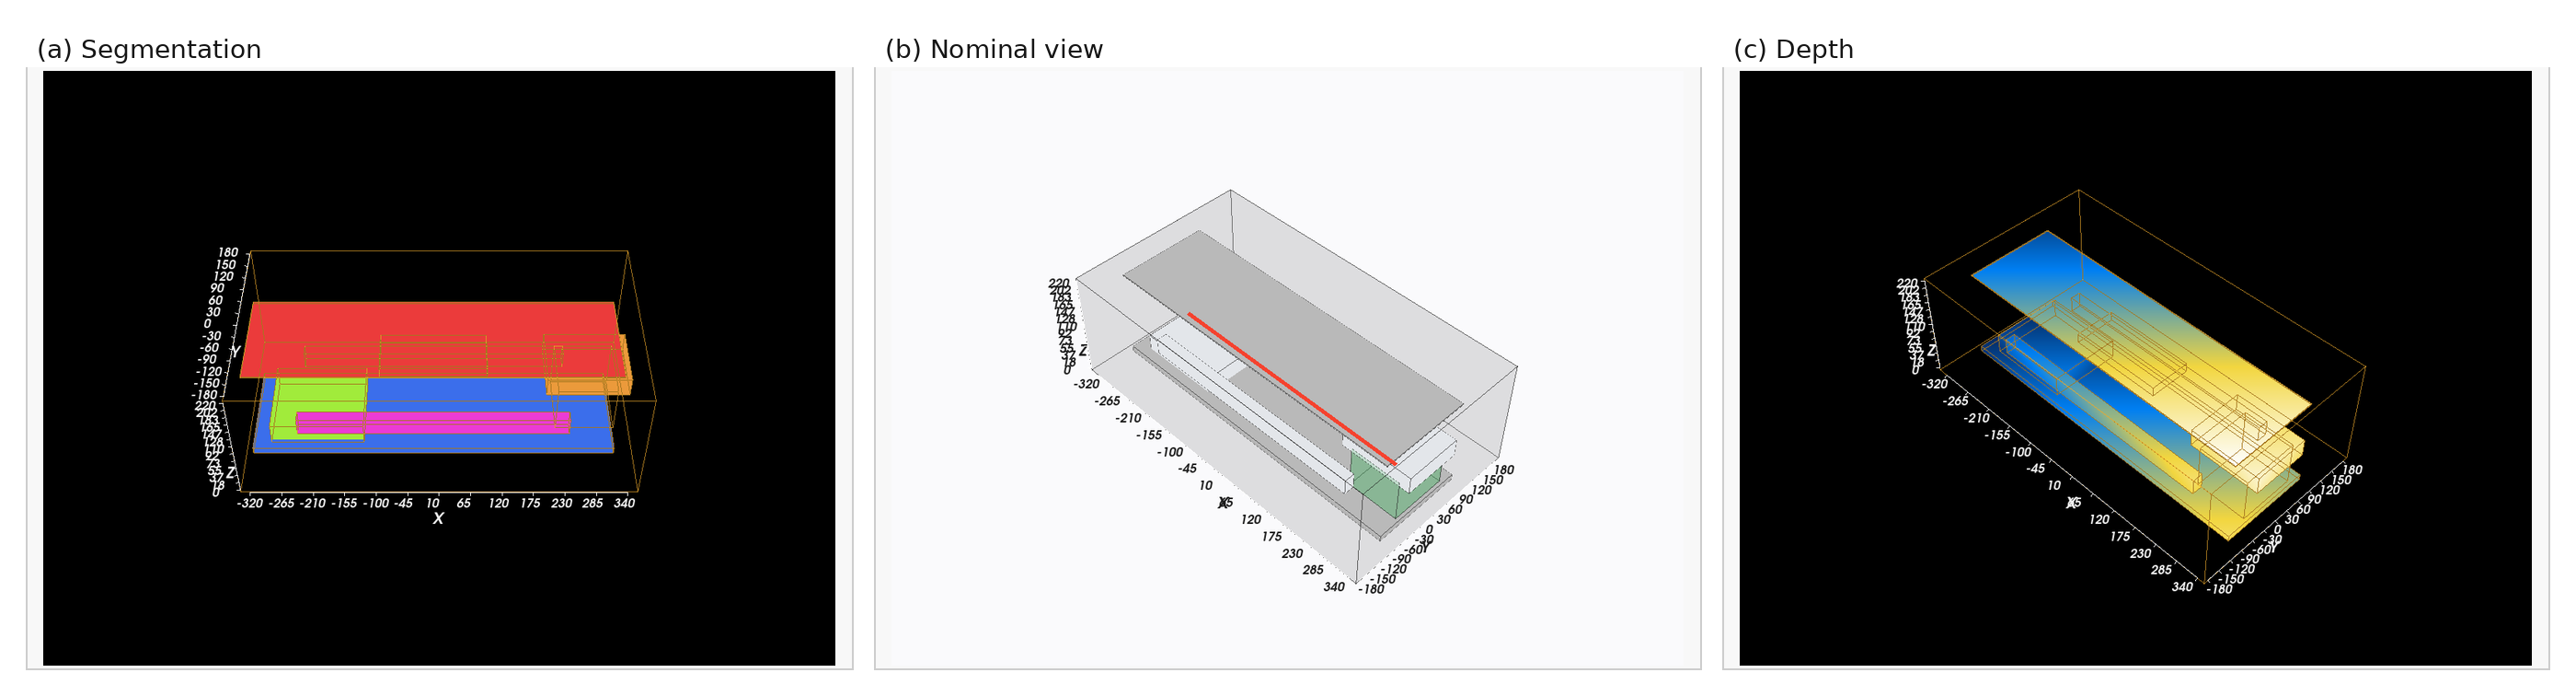
\includegraphics[width=0.98\linewidth]{appendix_render_collage.png}
\caption{Composite appendix render of the freestanding transfer mechanism, showing segmentation, a nominal perspective render, and depth information.}
\label{fig:appendix-render-collage}
\end{figure}

\end{document}
